%\documentclass[floatfix,11pt]{revtex4}
\documentclass[floatfix,11pt]{article}
\usepackage{color}
\usepackage{graphicx}
\usepackage{bm}
\usepackage{amsfonts}
\usepackage{mathrsfs}
\usepackage{amsmath}
\usepackage{amssymb}
\usepackage{setspace}
\usepackage{wrapfig}
\usepackage{fancyhdr}
\usepackage[labelfont=bf]{caption}
\usepackage{enumerate}
\usepackage{enumitem}
\usepackage{array}
\usepackage{natbib}
% \usepackage{pdfpages}
\newcolumntype{C}[1]{>{\centering\let\newline\\\arraybackslash\hspace{0pt}}m{#1}}

%----- Letter ----
\textwidth  = 6.5in
\textheight = 8.8in

\oddsidemargin = -0.in
\evensidemargin = 0.0in
\topmargin = -0.5in
\headheight = 0.5in
\headsep = 0.2in
\footskip = 0.4in

%%%%    HEADER     %%%%
\renewcommand{\headrulewidth}{0.75pt}
\pagestyle{fancyplain}
%\lhead{\small\textit{Mapping galaxies in spectral space}}
%\rhead{\small\textit{PI: Marina Meila}} 
\fancypagestyle{plain}

%%%%    FOOTER     %%%%
\renewcommand{\footrulewidth}{0.75pt}
\fancyfoot[LO]{\small\textit{DE-FOA-0002501}}
\fancyfoot[CO]{}
\fancyfoot[RO]{\small\textit{Page \thepage}}

%%%%%% my commands   %%%%%%


\newcommand{\dist}{{\rm dist}}
\newcommand{\epsi}{\varepsilon}
\newcommand{\D}{D}
\newcommand{\tily}{\tilde{y}}
\newcommand{\yg}{y_g}
\newcommand{\ygp}{y_{g'}}
\newcommand{\xg}{x_g}
\newcommand{\xgtrue}{x_{g}^{true}}
\newcommand{\xgptrue}{x_{g'}^{true}}
\newcommand{\xgf}{x_{g,l}}
\newcommand{\xgpf}{x_{g',l}}
\newcommand{\xgp}{x_{g'}}
\newcommand{\sigg}{\sigma_g}
\newcommand{\siggf}{\sigma_{g,l}}
\newcommand{\siggp}{\sigma_{g'}}
\newcommand{\siggpf}{\sigma_{g',l}}

\newcommand{\ml}{ML}
\newcommand{\sklearn}{{\tt scikit-learn}}
\newcommand{\mmani}{{\tt megaman}}
\newcommand{\gmani}{{\tt GigaMan}}

\newcommand{\comment}[1]{}
\newcommand{\mmp}[1]{\textcolor{blue}{MMP:#1}}
\newcommand{\bit}{\begin{itemize}}
\newcommand{\eit}{\end{itemize}}


\begin{document}
%\begin{center}
\vspace{-0.5em}
\vspace{-.25cm}
\centerline{\gmani:Embedding high-dimensional data with state of the art statistics}
\centerline{\textbf{PI: Marina Meila}, Professor of Statistics}

\centerline{University of Washington}
% Department of Statistics, Box 354322, Seattle WA 98195-4322, 
\centerline{Phone: 206-543-8484,  {\tt mmp@stat.washington.edu}}

\centerline{{\textbf DE-FOA-0002501}}
\\
\line(1,0){450}
%\end{center}
\singlespacing
\vspace{-.25cm}
\noindent\begin{tabular}{lll}
\multicolumn{3}{c}{Examples of data reduction by low dimensional embedding and smoothing}\\
\hspace{-2em}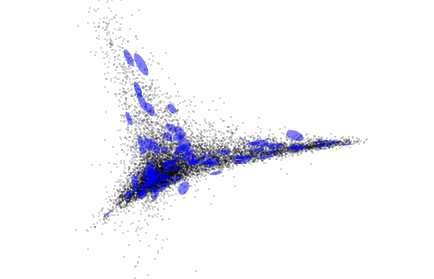
\includegraphics[width=2.in,height=1.4in]{Figures/word2vec_rmetric_plot_noaxis_trim.png} &
%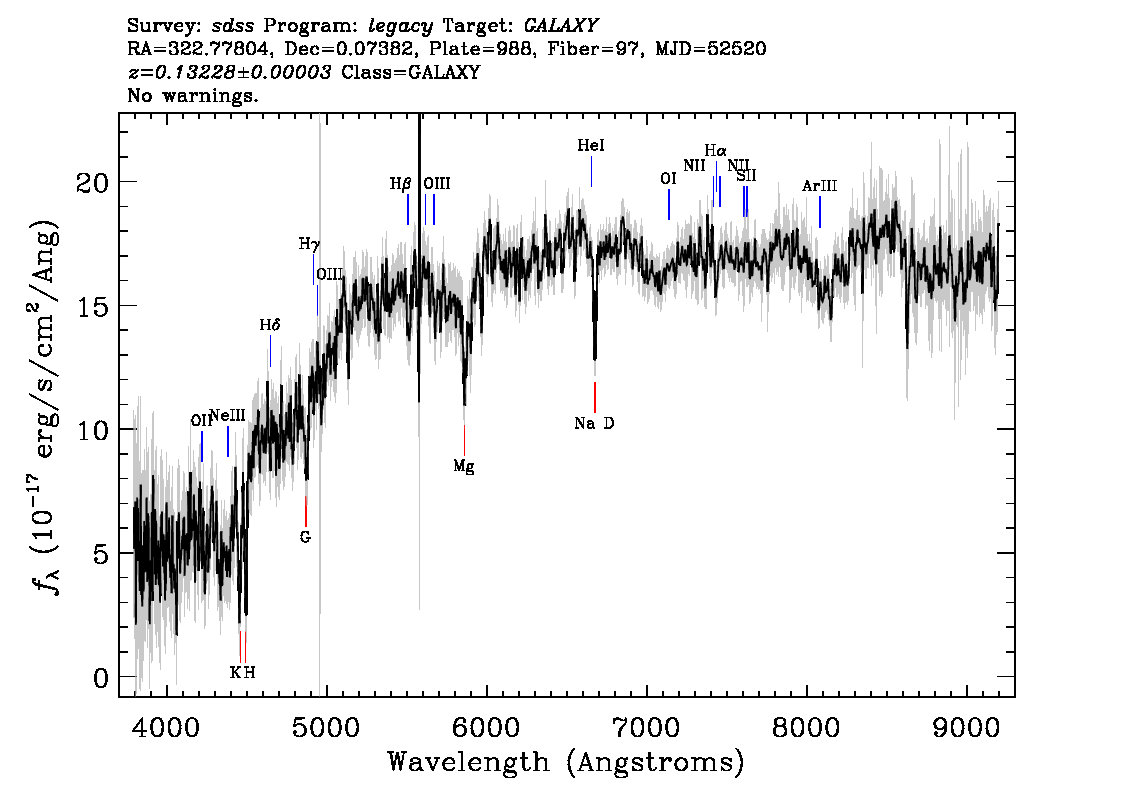
\includegraphics[width=2.2in]{Figures/specById_asp.png} & 
\hspace{-3.5em}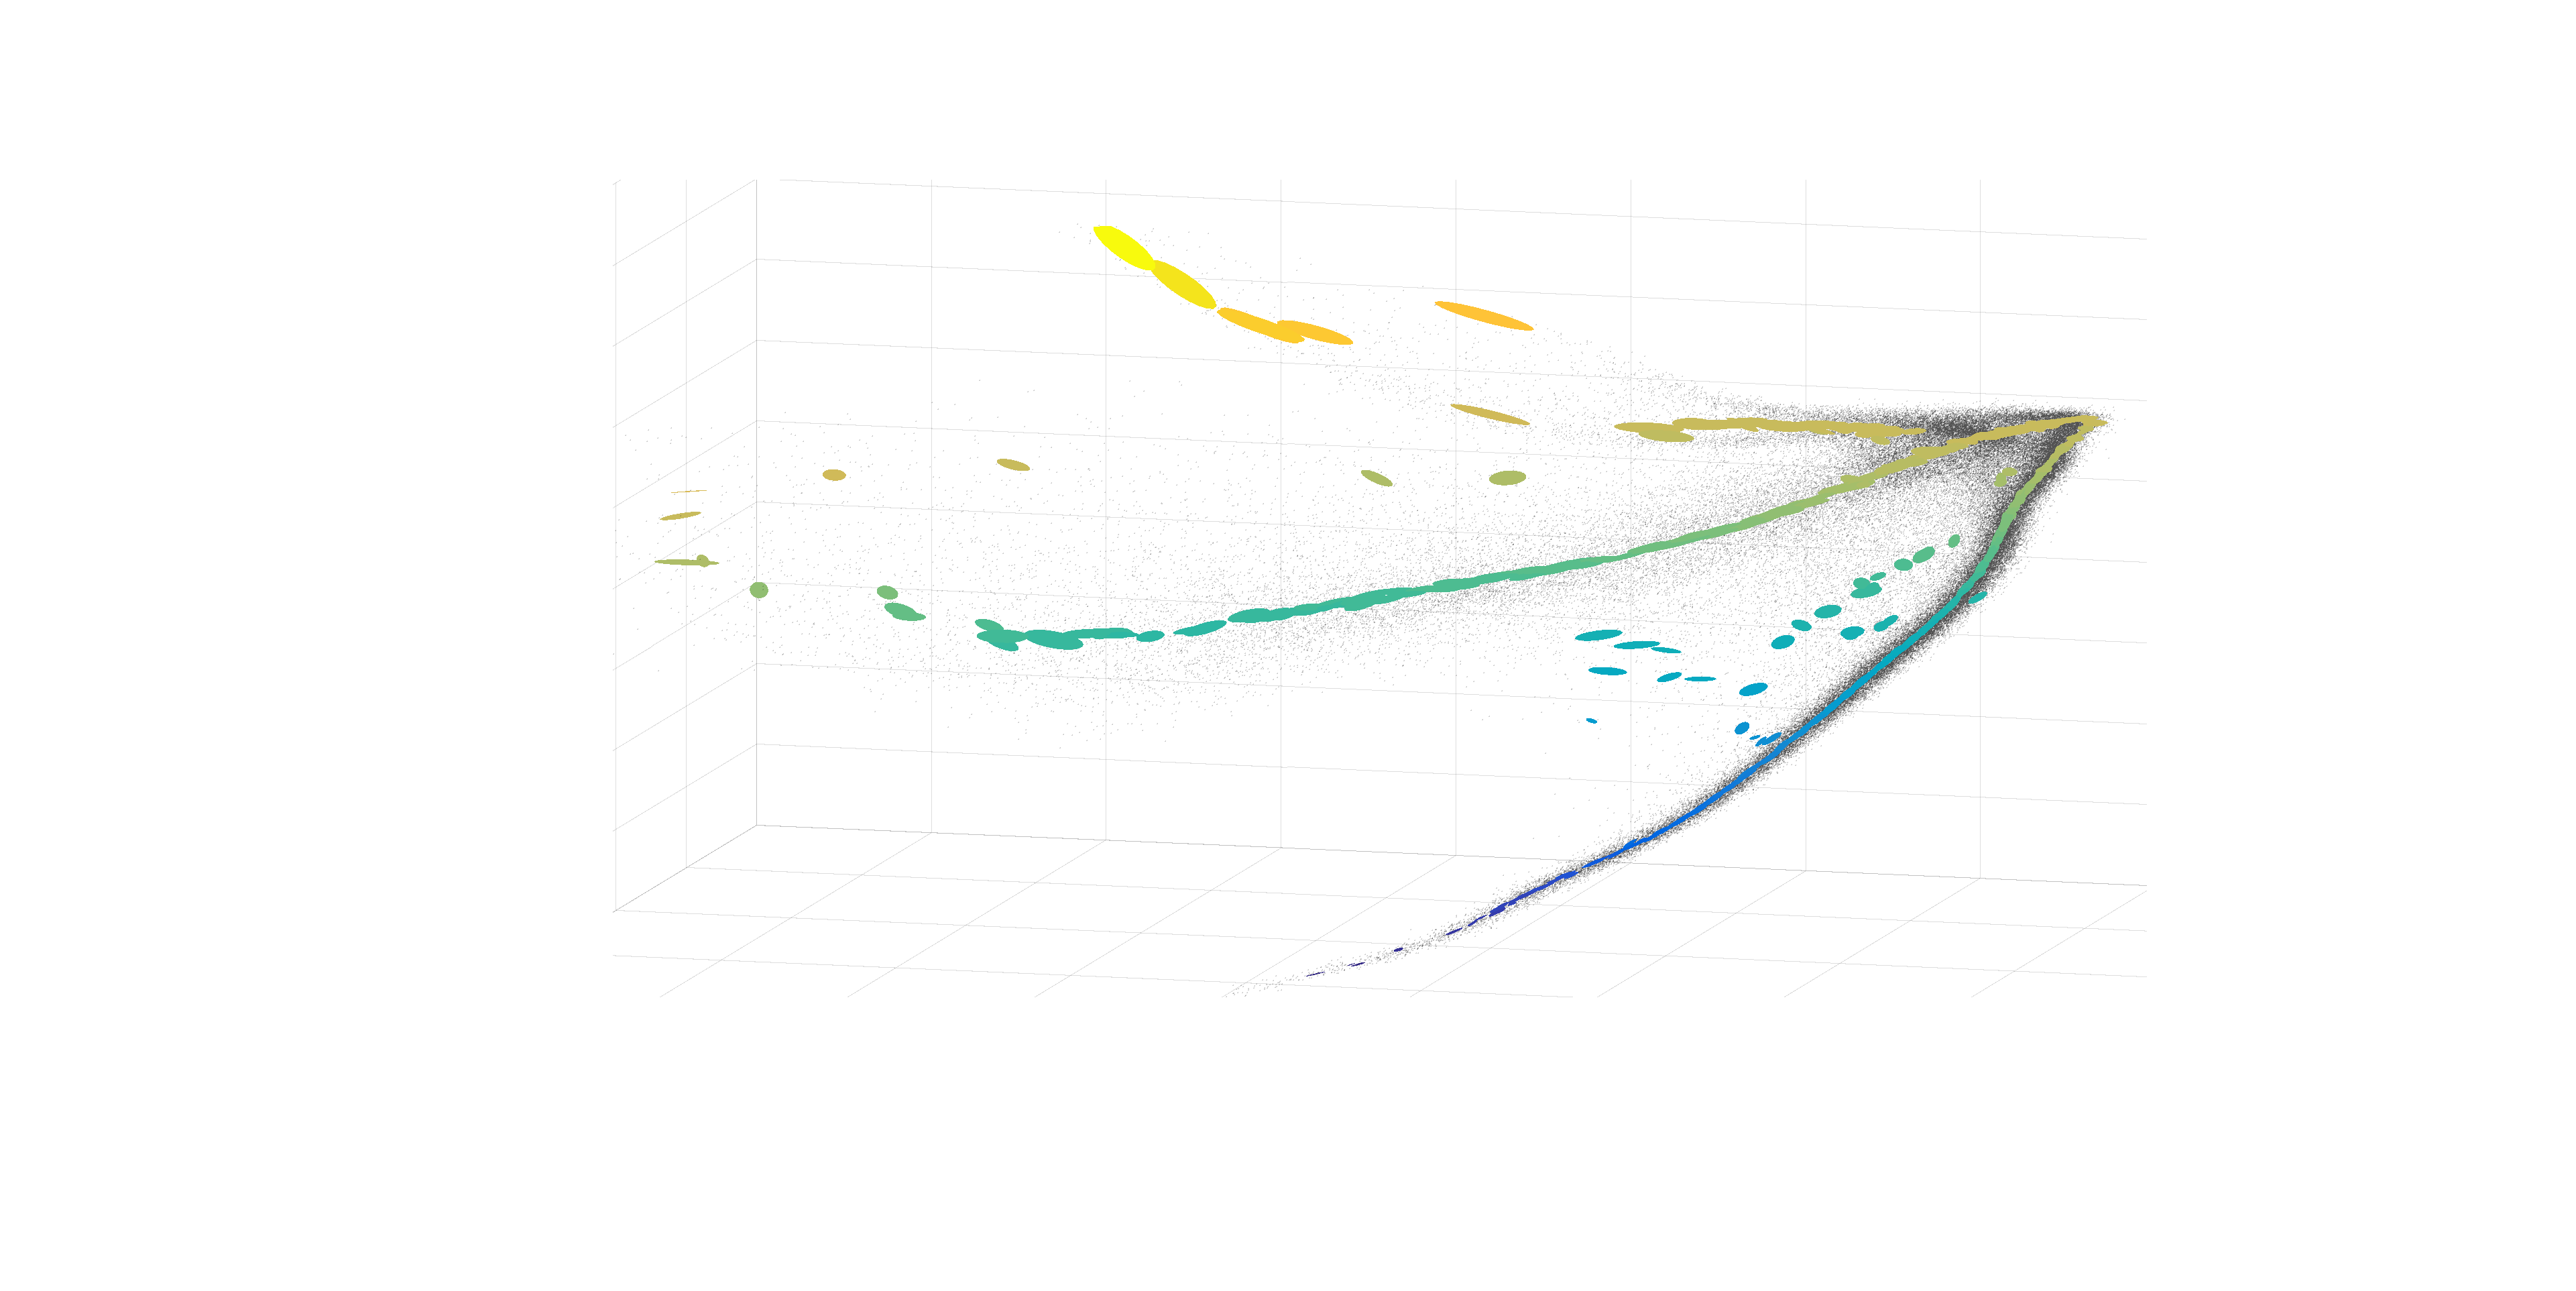
\includegraphics[width=2.5in,clip=]{Figures/spectrum_data_before-trim.pdf} 
&
\includegraphics[width=2.5in,clip=]{Figures/smoothed_velocity_field_alpha_50.pdf}\\
\multicolumn{3}{l}{
%\parbox[t]{4.5in}{%
\parbox[t]{\textwidth}{%
{\bf Left:} 3D embedding of 3,000,000 English phrases represented in 300 dimensions from {\tt https://code.google.com/archive/p/word2vec/}; {\bf middle:} 3D embedding of 660,000 spectra of galaxies from {\tt www.sdss.org} with 3750 wavelengths; {\bf right:} smoothed velocity field of 20,000 ocean buoys from {\tt https://www.ndbc.noaa.gov}}}
\\
\end{tabular}
\begin{tabular}{llll}
\multicolumn{3}{c}{Current widely used embeddings introduce artefacts}
&
\parbox[t]{1.5in}{\hspace{-0.5em}Measuring distortion \cite{2013arXiv1305.7255P}}
\\
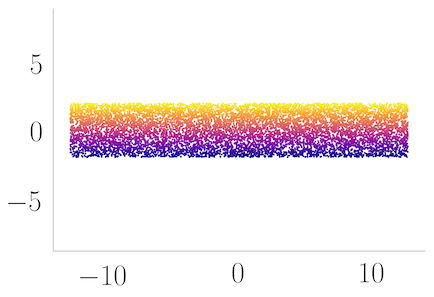
\includegraphics[width=1.6in]{Figures/D1_original_data.png} &
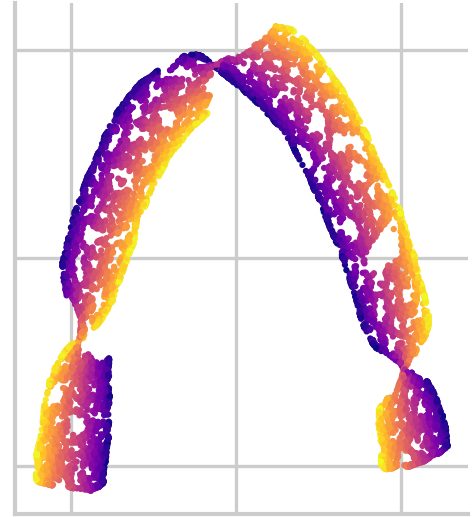
\includegraphics[width=0.8in]{Figures/umap_mindist_comp.png} &
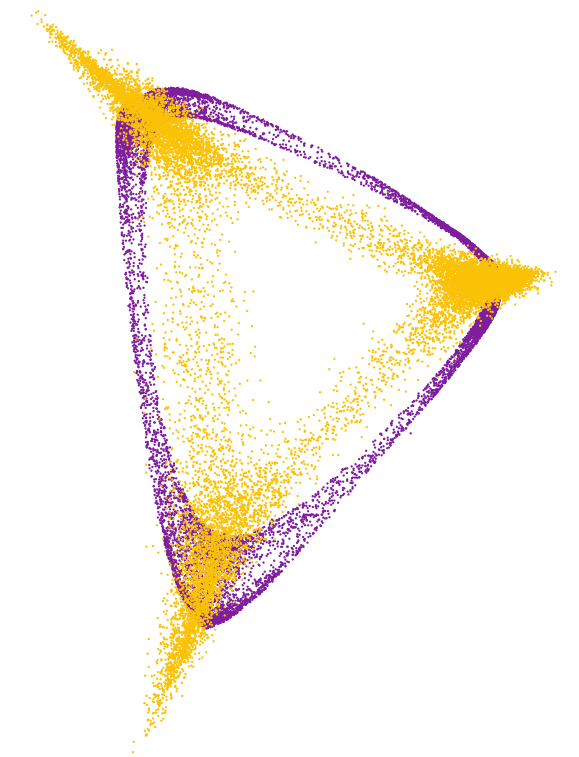
\includegraphics[width=1.2in,angle=90]{Figures/geometric_vs_normalized.png}
&
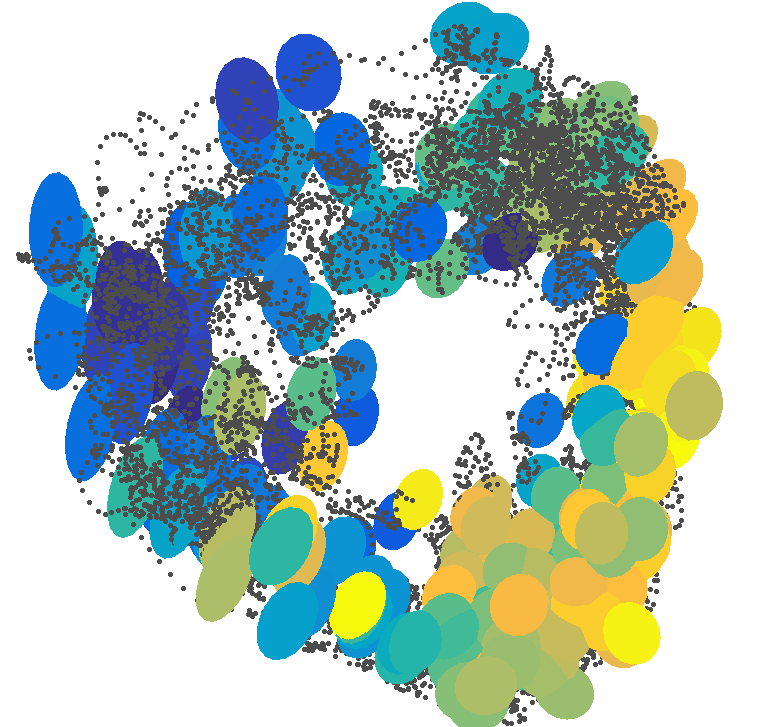
\includegraphics[width=1.4in,angle=90]{Figures/aspirin-postclu1-phi234Rmetric-tau22.png}
\\
\multicolumn{3}{l}{\parbox{4.3in}{{\bf Left, middle:} Embedding of a 2D strip by UMAP, showing 4 clusters inexistent in the original data; {\bf right:}  embeddings of molecular configurations of ethanol showing distortion (purple) and degeneracy (yellow); the original data is a torus.}}
&\parbox[t]{1.9in}{Embedding distortion size and direction is displayed as ellipses.}\\
\end{tabular}

{\bf Objective}: \gmani, a non-linear dimension reduction toolbox
in python, that scales to data matrices of order $n\times p \sim
10^{12}$, by vertically incorporating the state of the art in the mathematics and statistics of high dimensional geometric learning, and specifically in fast approximate {\em near neighbor (NN)} search.

\textbf{Motivation and challenges} Data in the form of
high-dimensional ``point clouds'', \comment{such as spectra of galaxies \comment{(with
dimension given by the number of spectral wavelengths)}, spatial
locations of the atoms in a molecule \comment{(with dimension given by the number atoms $\times$ spatial dimension 2 or 3)}, the state space of a dynamical system, as well as data for which a {\em distance} between observations can
be calculated, such as biological sequences, words and phrases, job
descriptions, images. } as exemplified in the figures above, is ubiquitous.
%
Often, the physical processes underlying these observations have
fewer degrees of freedom than the data dimension, and they can be
modeled by {\em manifolds} and vector fields thereon, achieving
significant data reduction, as well as noise removal and better understanding of the intrinsic degrees of freedom of the system. This class
of methods is known as (non-linear) {\em  embedding} methods.

\comment{ Embeddings know-how is relevant other data reduction in approaches too. One is smoothing the data, by projecting it onto a local manifold; the other is subsampling the regions where the data is too dense, and summarizing the local geometry by means of indexing, meta-information, or core-sets.}

\comment{Data reduction for the sciences must come with guarantees of
  reproducibility (e.g. outputs not sensitive to initialization of
  algorithm), stability (outputs not sensitive to variations in
  sample), as well as with rigurous methods to quantify the loss of
  information and the variability of the result, and with
  guarantees of preserving desired properties/features/(geometric)
  characteristics}

Estimating non-linear geometry is hard in statistical and mathematical terms. This is why na{i}ve embeddings, not grounded in theory, are {\em biased}, introducing distortions, or even {\em inconsistent}, tending to unreasonable/degenerate limits when $n\rightarrow \infty$. The statistical methods needed to analyze the properties of embedding algorithms and to design consistent, unbiased, ones are being developed. For example, \cite{2013arXiv1305.7255P} introduce a method based on Riemannian geometric concepts to calculate and to correct distortions in embeddings (see Figure). This method guarantees that the low dimensional embedding is isometric (preserves the intrinsic geometry) of the original, and can also detect degeneracies. 
However, (1) existing theory is too technical to be accesible to most scientists and engineers; (2) the theorems depend on unspecified constants and on properties of the data. To bring them to be relevant to science {\em one must develop methods to measure and test} if the theoretical conditions hold. One must also select those theoretical results that relie on testable assumptions, and that best fit the statistical structure of the problem. \comment{For example, the embedding algorithms must adapt to  the density of molecular configurations in state space can vary exponentially, or to the variation of measurements noise with red-shift and wavelength in spectrographic observations of galaxies, and exploit these properties, whenever possible.}

(3) Further scaling up embedding algorithms by a factor of 1000 or more, depends crucially on accelerating {\em approximate} NN \cite{charikarKapralovNouriSiminelakis:kde20} search. The first methodological focus of this work is ensuring that statistical guarantees for embedding algorithms still hold when approximate NN is used. The second is to translate these guarantees into uncertainty quantifications for actual data. 

\textbf{What we will do}
\\
{\em Methods (MM)} for approximate near neighbor search, data indexing and subsampling, statistically suitable for non-linear embedding. The methods will be grounded in state of the art statistical and CS theory, and will come with error estimates, noise and information loss measures, and diagnosis methods (e.g. for degeneracy). [Responds to Priority Research Directions (PRD) (1,3)]\\
{\em Theory (MM)}  Original research on how to measure/test from data when theoretical conditions apply; to choose the optimal embedding method for a particular data, to derive what guarantees can be obtained from theory for the reduction of a real data set. [PRD (1,3)]
 \\
{\em Specific sciences (DB,AC,ZI,MJ)} have specific data statistitics (e.g. variations in data density, noise properties). We will specialize the generic data reduction methods above on data properties relevant to astronomy, astrophyisics, chemistry, and bio-engineering.[PRD (4)]\\
{\em Software (AVM$+$DB,AC,ZI,MJ,MM)} Release of a suite of open-source python packages implementing the above methods, and specializing them for the Legacy Survey of Space and Time (LSST) data (40B points $\times$ 10,000 dimensions), and Molecular Dynamics simulations. 
Platforms: generic clusters like the AWM, Hyak, and Leadership Computing Facilities (LCF), such as {\tt Aurora, Polaris}. [PRD (4)]
\comment{ (3) Computationally, finding neighbors of a point in high dimensions is the bottleneck, and approximate methods must be proved to not compromise the consistency of the embedding algorithm.
These are the barriers to the adoption of the state of the art knowledge in data embedding,  and herein lies our main contribution. }

\underline{\bf Team} %Team of exceptional depth and breadth.
PI Meila is uniquely situated to successfully carry out this work. She is fluent in the statistical and theoretical CS advances, and can critically judge their relevance. She has a 10 year long track record of addressing critical geometric learning problems by novel methods grounded in theory \citep{2013arXiv1305.7255P,MChen:ies-neurips19}. Her group maintains \mmani, an open-source package capable of applying these to millions of data points, and has collaborations with ALCF and Sppexa (German Exa Scale Computing Consortium) to expand these to HPC environments.

All team members are experts in data science and interdisciplinary research, and have collaborated with the PI. DB and AC are respectively Director and Director of Research for the eScience Institute and experts in cosmology, respectively chemistry, bio-engineering, ZI is the Project Scientist for the LSST, MJ is Director of the DIRAC Institute for Cosmlogical and Astrophysical Research. 
\comment{Meila, Connolly and Ivezic collaborated on more than five grant proposals; Meila and Beck collaborated on four grant proposals, two of them funded by the DE under FOA .... Meila and Vasquez-Mayagoitia collaborated on the ALCF Grant .... As part of this collaboration, the software \mmani~was ported on the Theta, and UW student Yu-chia Chen visited ALCF. \mmani~originated in the first Data Science Incubator as a collaboration between Meila and Jake VanderPlas. }
\comment{
Dr. Marina Meila is Professor of Statistics with adjunct appointments in Computer Science and Electrical Engineering at UW. Her primary expertise is in machine learning, specifically in statistical learning, high-dimensional inference and big data. She has widely recognized contributions to learning in graphical models, spectral clustering,37 non-linear dimension reduction,38 Bayesian statistics,39 and sparse estimation. Her group developed the open source Python package “megaman”40 (over 45K downloads) which performs dimension reduction and other ML tasks on millions of points in thousands of dimensions. She has authored 108 publications and has an h-index of 36.
, the University of Washington’s central institute for data science and machine learning. He directs a team that develops new data science methods and software in coordination with researchers across the pacific northwest. He is an expert in the development and application of open source tools for data science and machine learning in areas such as energy, environment, and health. He is the author over 80 peer reviewed publications with a h-index of 31.
}

\vspace{-1.1em}
\bibliographystyle{abbrv}
\bibliography{proposal}
\end{document}
\newpage
\centerline{\textbf{Senior Personnel}}
\vspace{1.5em}
\begin{tabular}{lllll}
  Last name & First name & Title & Institution\\
  \hline
Beck & David & Professor &  University of Washington & co-PI\\
Connolly & Andrew & Professor &  University of Washington& co-PI \\
Ivezic & Zeljko & Professor &  University of Washington& co-PI \\
Juric & Mario & Associate Professor &  University of Washington& co-PI\\
Meila & Marina & Professor & University of Washington& PI\\
Vasquez-Mayagoitia & Alvaro & Computational & Argonne National& co-PI\\
& &Scientist & Computing Facility&\\
\end{tabular}

\vspace{1.4em}
\centering{\textbf{Collaborators, Co-editors, and Graduate and Postdoctoral Advisors and Advisees of the PI and Senior/Key Personnel}}
\begin{tabular}{llll}

\end{tabular}


Molecular dynamics of hundreds of thousands and multi-million atom simulations are becoming more common in materials science and biochemistry, such kind of simulations are extremely data intensive, while storing and post-processing data is highly demanding in terms of CPU cycles and non-volatile memory. DOE has announced exascale capabilities in its Leadership Computing Facilities (LCF).  We will collaborate with LCF to accelerate post-processing exascale simulations and enable in-situ analysis. We would collaborate with ALCF to port Gigaman to use efficiently hardware accelerators and make the most of specialized architectures for data analysis.

DOE has announced exascale capabilities in its Leadership Computing Facilities (LCF), such as Aurora and Frontier. 

We would collaborate with ALCF to port Gigaman to use efficiently hardware accelerators and make the most of specialized architectures for data analysis in Aurora and Polaris.

ZI is the Project Scientist for the Rubin Obsevatory’s Legacy Survey of Space and Time (LSST).
LSST dataset can be described as a 10,000-dimensional space populated by 40 billion points
and thus will provide prime testing ground for new manifold algorithms proposed here.

